
\documentclass{article}
\usepackage[utf8]{inputenc}
\usepackage[english]{babel}
\usepackage{amsmath}
\usepackage{natbib}
\usepackage{graphicx}
\usepackage{hyperref}
\usepackage{caption}
\usepackage{epstopdf}
\usepackage{float}
%\epstopdfsetup{outdir=./}

\title{Growing Degree Days}
\author{\bf{CMSC6950 Project}\\\\Hanieh Marvikhorasani\\ Mahesh Kumar Reddy Pochamreddy\\ Jonathan Conway}
\date{\today}

\begin{document}


	\clearpage\maketitle
	\thispagestyle{empty}

\newpage

\section{ \bf Introduction}
The growing degree days (GDD) is a temperature index tool used in agriculture to predict the best planting season for a plant. GDD enhances predicting the best planting time of a crop to its maturity, in terms of high heat accumulated in the ground in regions conducive. GDD is used to predict and compare the growing rate of a plant from germination to yielding and predict future planting. Generally, GDD is calculated by adding the maximum (Tmax) and minimum (Tmin) temperature together dividing by two (2) and then subtracting the base temperature (Tbase).

\noindent When determining the GDD of a plant, each plant has a conducive temperature for development and so it has a base temperature (Tbase). The base temperature is the lowest temperature a plant can survive in. (Tbase) will be considered 0 degrees celcius for the calculation of GDD in this report.

\noindent The reference temperature for a given plant is the temperature below which its development slows or stops. For example, peas are planted during the cold season, where it has a reference temperature of 40 degrees fahrenheit while sweet corn and soybeans are planted during the hot season, where they have a reference temperature of 50 degrees fahrenheit.


\noindent 
Generally, GDD is calculated by adding the maximum (Tmax) and minimum (Tmin) temperature together dividing by two and then subtracting the base temperature (Tbase). 
When determining the GDD of a plant, each plant has a conducive temperature for development and so it has a base temperature (Tbase). The base temperature is the lowest temperature a plant can survive in. (Tbase) will be considered 0 $^{\circ}$C for the calculation of GDD in this report.


\section{ \bf Methodology}
\subsection{Data Collection}
Required  data  for  different  cities  have  been  obtained  from  the  given  website:
https://climate.weather.gc.ca.  Also needed columns including year, Min Temp,
Max  Temp  and  etc  have  been  extracted  for  the  selected  cities  and  this  data
have  been  used  to  create  the  plots  for  defined  tasks.   

\noindent The main data selected was the monthly data for 2016 from stations located in Montreal, Victoria, and Ottawa. This data was used to complete the required Minimum Core Tasks.

\noindent For the regression analysis performed for the Secondary Tasks, data from 1950 to 2010 was selected from a weather station in Montreal.

\noindent Data was also selected from unique stations on the island on the Newfoundland based on the 6 different geographic regions. This data spans 10 years and covers the years 1995-2004. This data was used to compile the necessary files for the Final Task analysis which will be elaborated further in this report. 


\subsection{ \bf Scientific Results for Minimum Core Tasks}

\begin{enumerate}
\item For our Core Tasks, we chose data from Montreal, Ottawa, and Victoria for the year 2016(Fig. \ref{Canada})

\begin{center}
\begin{figure}[H]
\centering
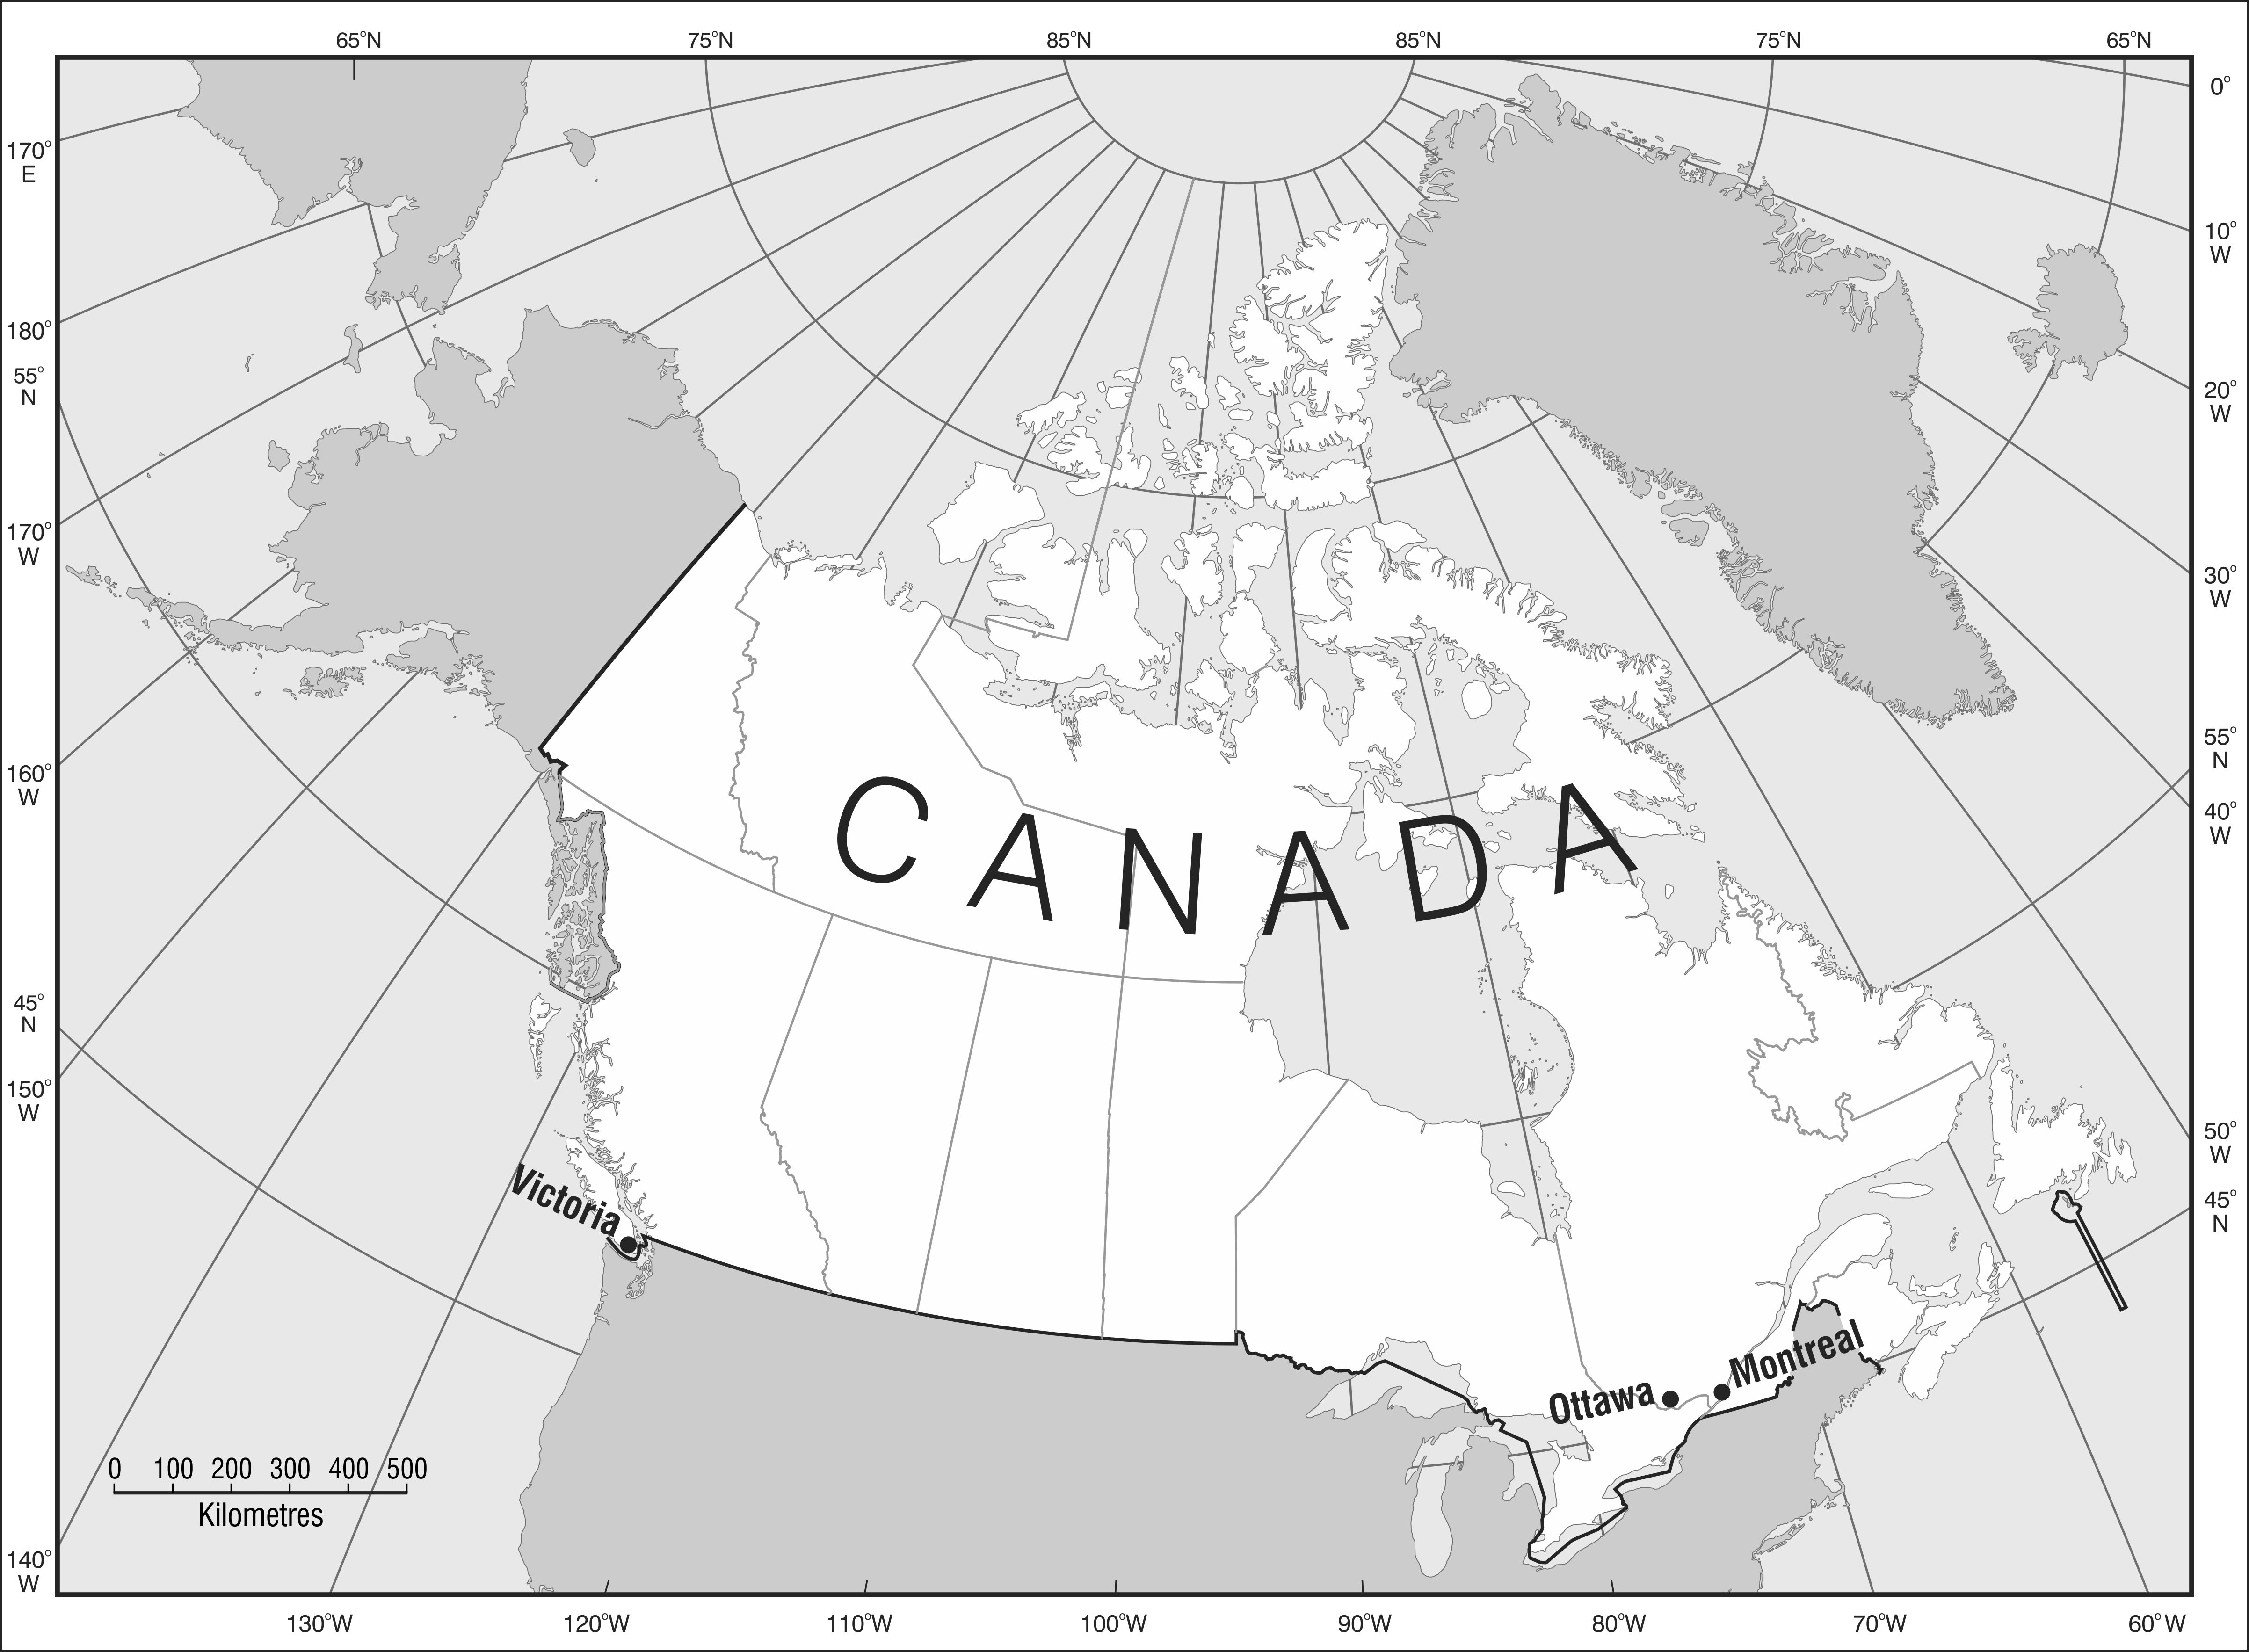
\includegraphics[width=3.25in]{Canada_final.jpg}

\caption{}
\label{Canada}
\end{figure}
\end{center}

 
\item  Showing annual cycle of min/max daily temperatures for selected Canadian cities. We did this analysis on Montreal, Victoria, and Ottawa for 2016.(Fig. \ref{min-max})
\begin{center}
\begin{figure}[H]
\centering
\includegraphics[width=3.25in]{../data/MinMaxPlot.png}

\caption{Min/Max temps for Montreal, Ottawa and Victoria in 2016}
\label{min-max}
\end{figure}
\end{center}

\item Calculating and storing GDD to analyze via the command line.
\item  Showing accumulated GDD vs time for some selected cities 
(Fig. \ref{accumulatedGdd})
\begin{center}
\begin{figure}[H]
\centering
\includegraphics[width=3.25in]{../data/3932accGdd.png}

\caption{accumulated GDD }
\label{accumulatedGdd}
\end{figure}
\end{center}
\end{enumerate}


\subsection{ \bf Scientific Results for Secondary Tasks
 }
\begin{enumerate}
\item Create a plot showing GDD

\item Standalone Bokeh Plots \ref{bokeh})

\begin{center}
\begin{figure}[H]
\centering
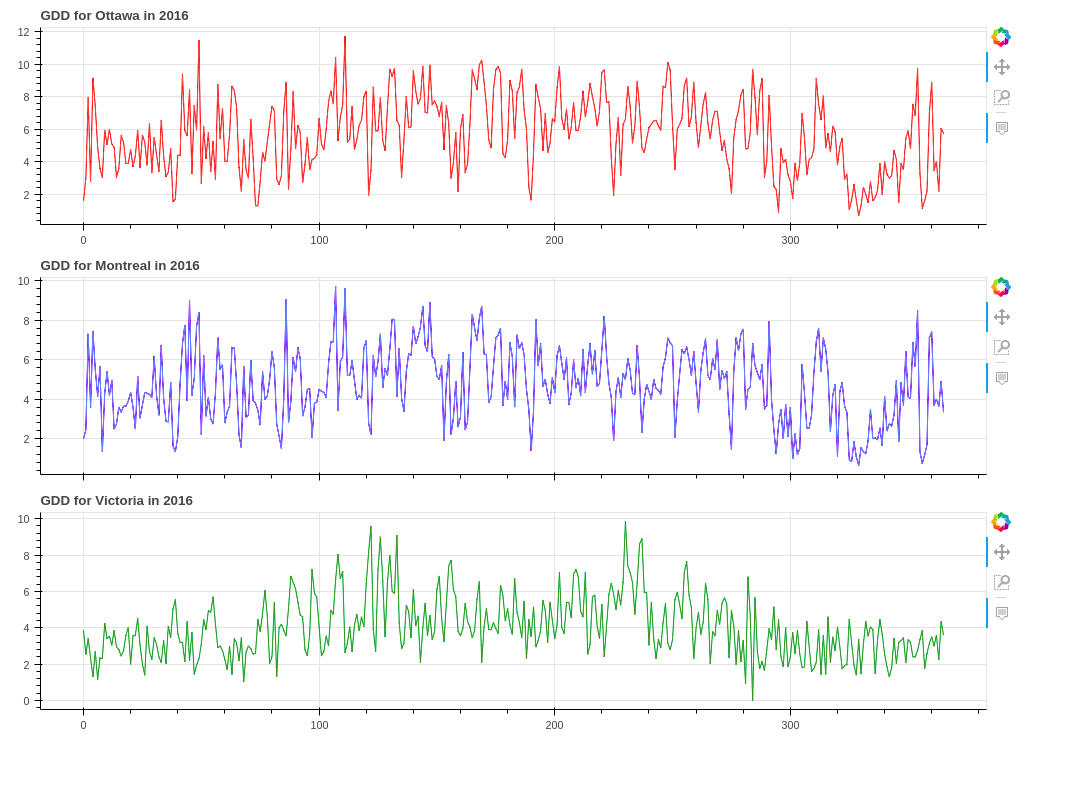
\includegraphics[width=4.5in]{../docs/BokehPlot.png}


\caption{Bokeh plot }
\label{bokeh}
\end{figure}
\end{center}

\item Comparing GDD year-over-year for Montreal between 1950 to 2010(Fig. \ref{regression}).

\begin{center}
\begin{figure}[H]
\centering
\includegraphics[width=3.25in]{../data/LinReg.png}


\caption{Regression between total GDD and years}
\label{regression}
\end{figure}
\end{center}



\subsection {\bf Final Tasks} 
The island of Newfoundland was divided into 6 geographic regions; North, South, East, West, Central, and The Avalon(Fig. \ref{regions}).

\begin{center}
\begin{figure}[H]
\centering
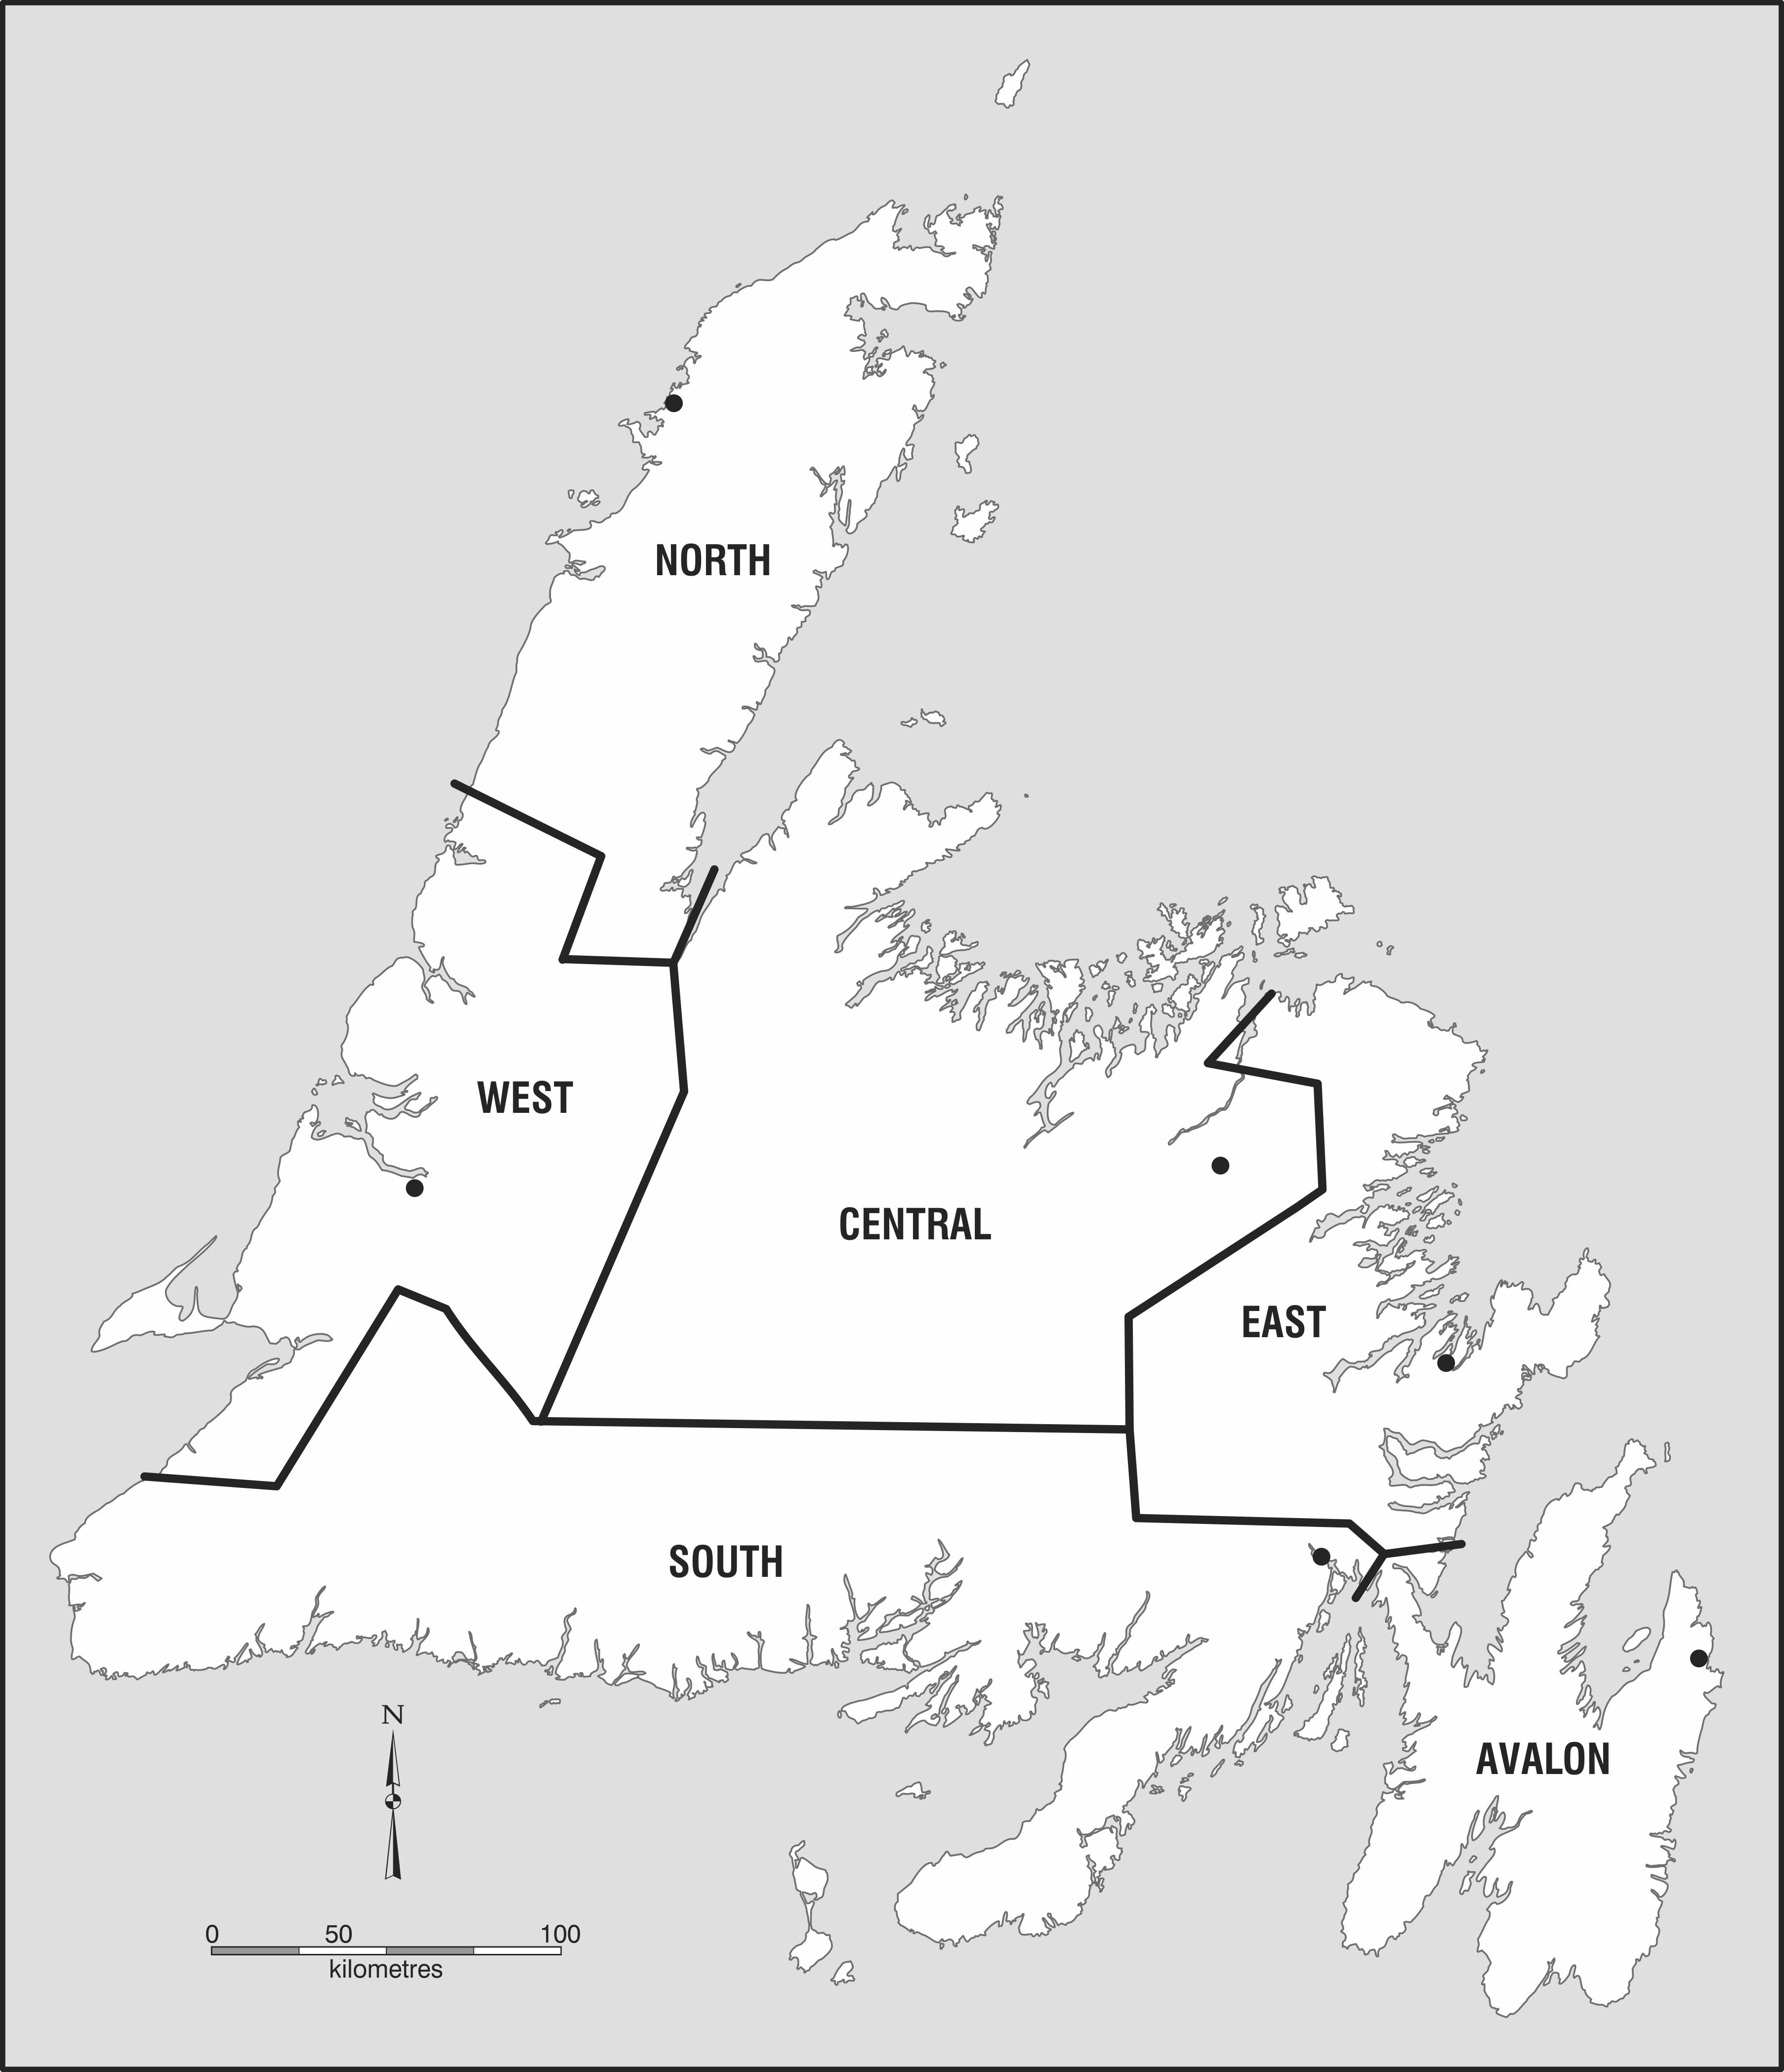
\includegraphics[width=3.25in]{../docs/Island_of_Newfoundland_Regions_final.jpg}
\caption{Newfoundland regions}
\label{regions}
\end{figure}
\end{center}

A station from each region was selected: Plum Point (North), Swift Current (South), Charleston (East), Corner Brook (West), Gander (Central), St. John's (The Avalon) (Fig. \ref{selected_stations}).
 
 \begin{center}
 \begin{figure}[H]
 \centering
 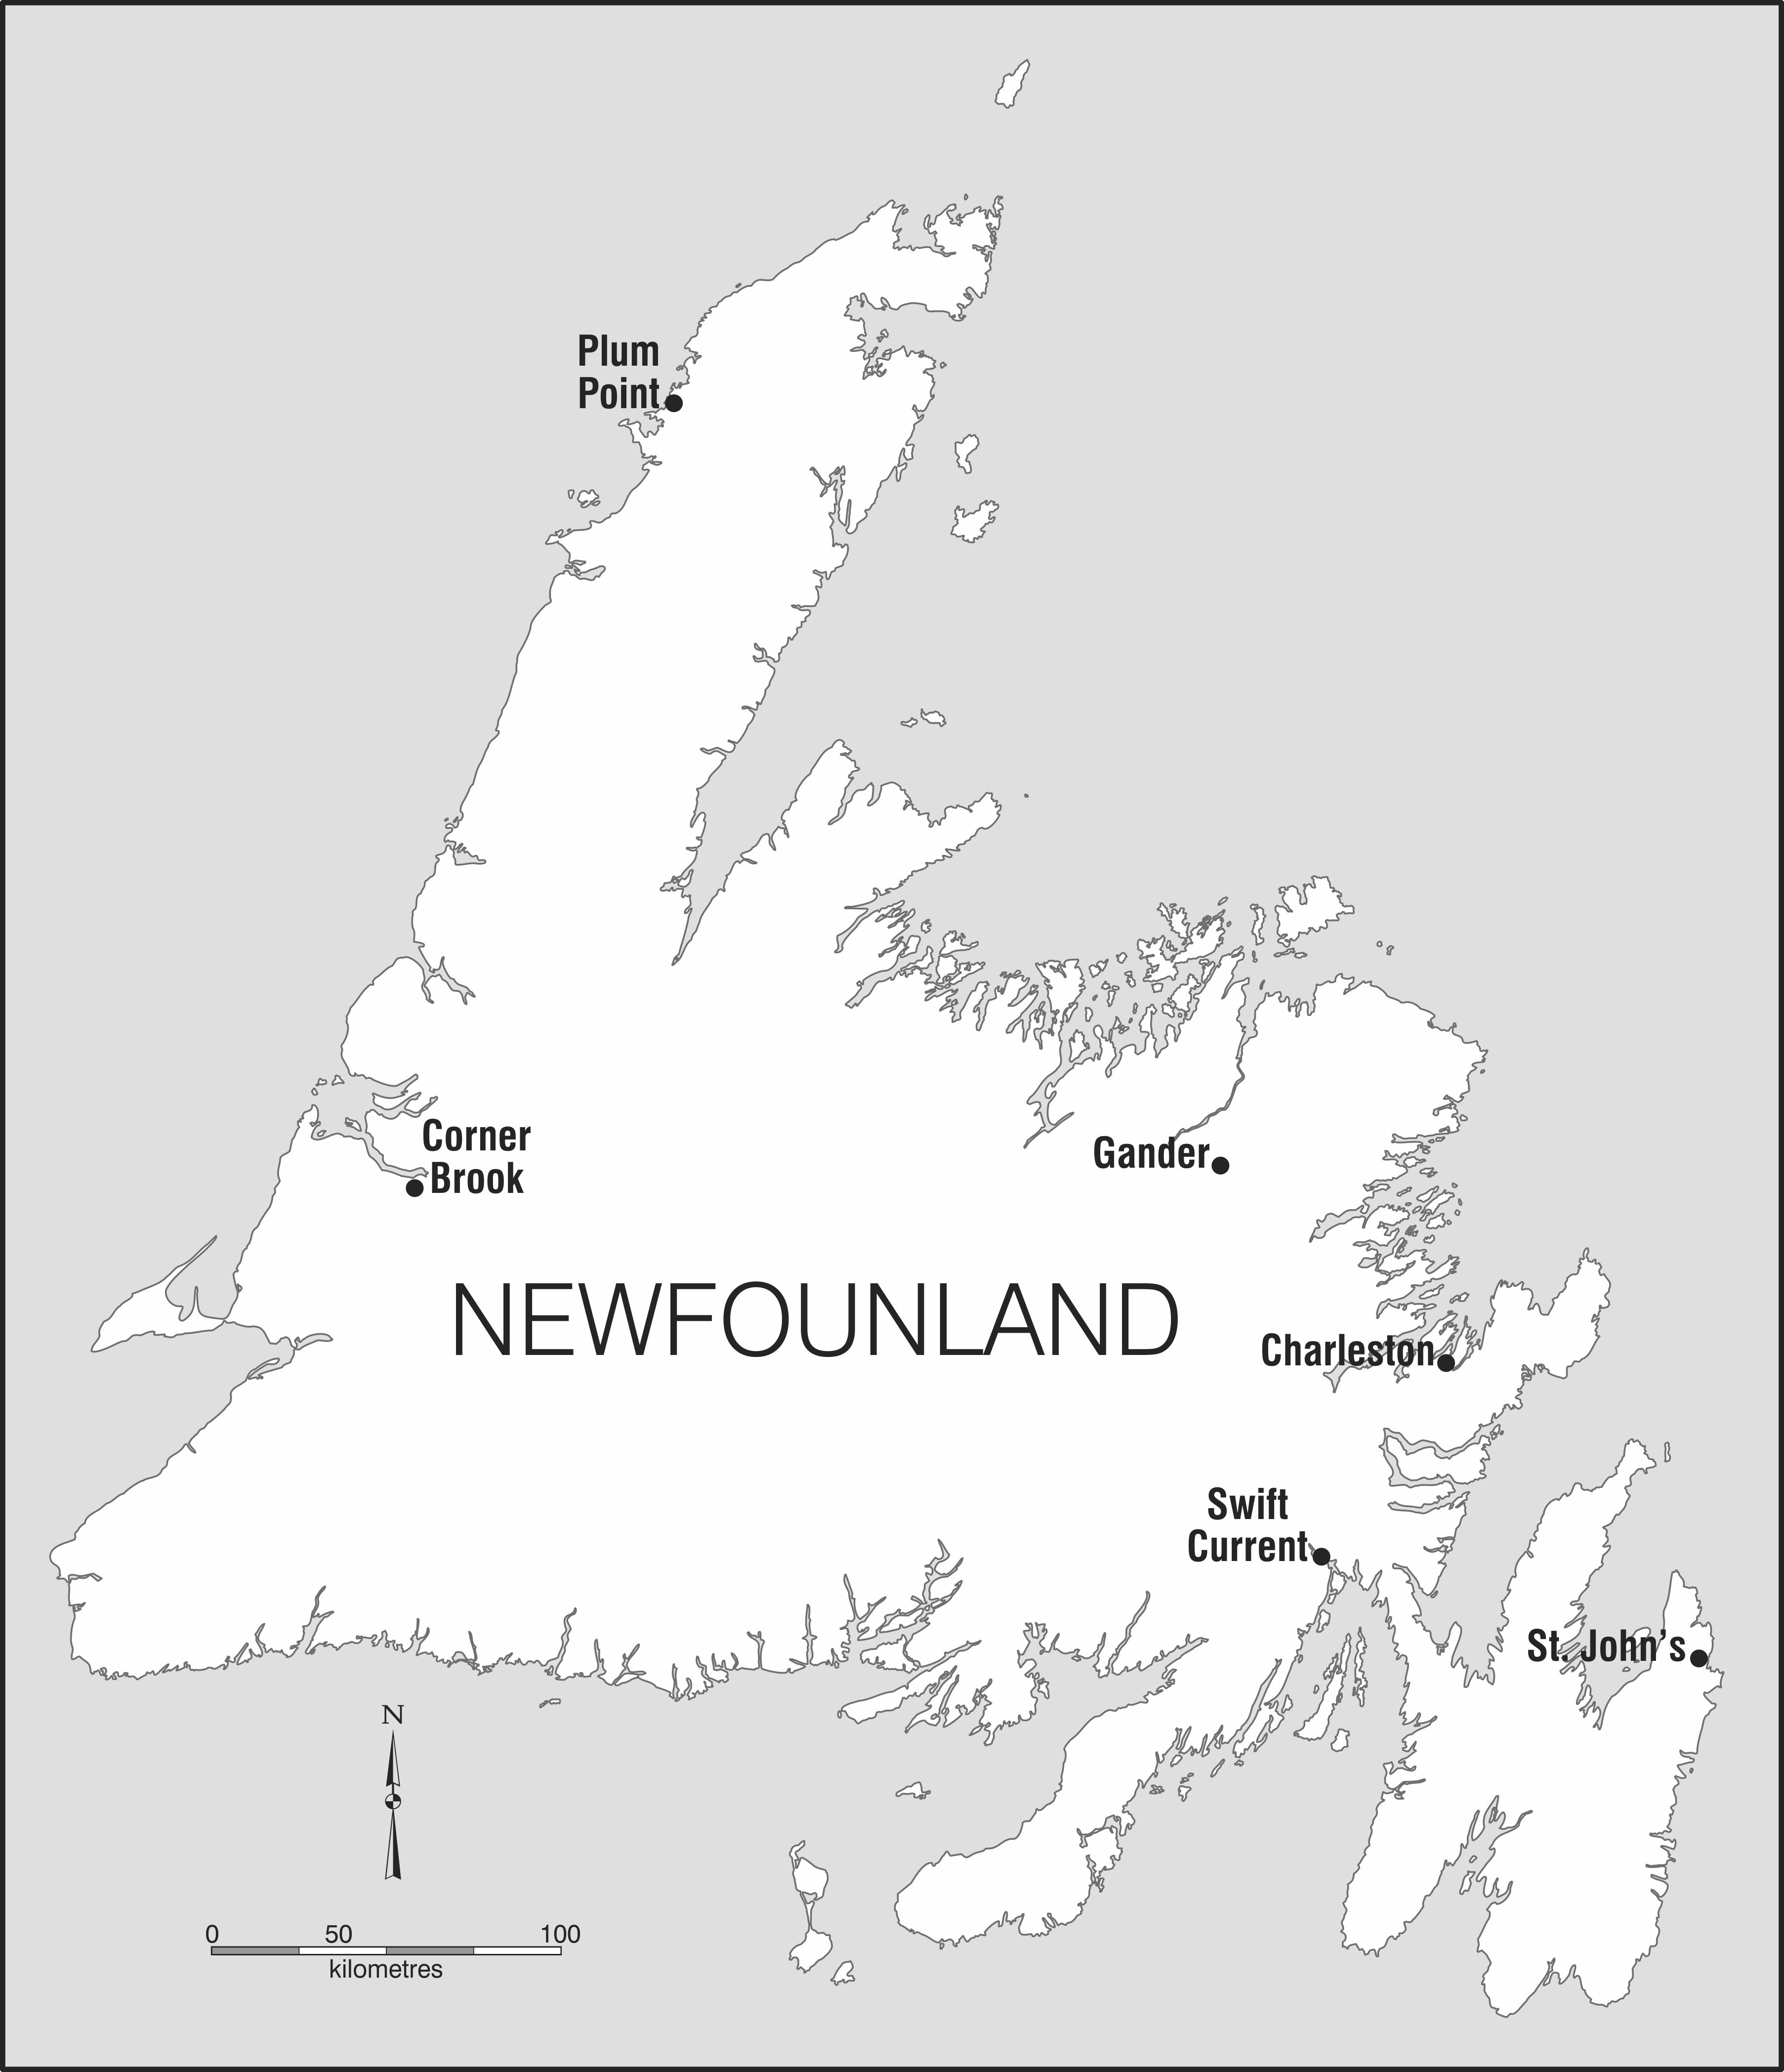
\includegraphics[width=3.25in]{../docs/Island_of_Newfoundland_final.jpg}
 \caption{Selected stations in Newfounland }
 \label{selected_stations}
 \end{figure}
 \end{center}

The 10 Year Average Annual GDD was calculated and compared to the minimum GDD for 3 types of wheat[1]. From the analysis, based solely on GDD, parts of Newfoundland could sustain wheat production(Fig. \ref{wheat}).

 \begin{center}
 \begin{figure}[H]
 \centering
 \includegraphics[width=3.25in]{../data/nlwheatplot.png}
 \caption{Wheat growth analysis based on GDD in Newfoundland }
 \label{wheat}
 \end{figure}
 \end{center}
 
 Using the 10 Year Average Annual GDD calculation again, the results were compared to the minimum GDD for 6 types of seeds[2]. From the analysis, based solely on GDD, parts of Newfoundland could sustain wheat production(Fig. \ref{seeds}).
 

\begin{center}
\begin{figure}[H]
\centering
\includegraphics[width=3.25in]{../data/nlseedplot.png}

\caption{Seeds growth analysis based on GDD in Newfoundland}
\label{seeds}
\end{figure}
\end{center}


\end{enumerate}

\begin{thebibliography}{99}
	\bibitem{wheat1}
	http://store.msuextension.org/publications/agandnaturalresources/mt200103ag.pdf
	\bibitem{seed1}
	http://store.msuextension.org/publications/agandnaturalresources/mt200103ag.pdf
\end{thebibliography}
	
 
\end{document}
